\setchapterstyle{kao}
% \setchapterpreamble[u]{\margintoc}
\chapter{Research and implementation}
\label{ch:problem}

\begin{figure}[hb]
    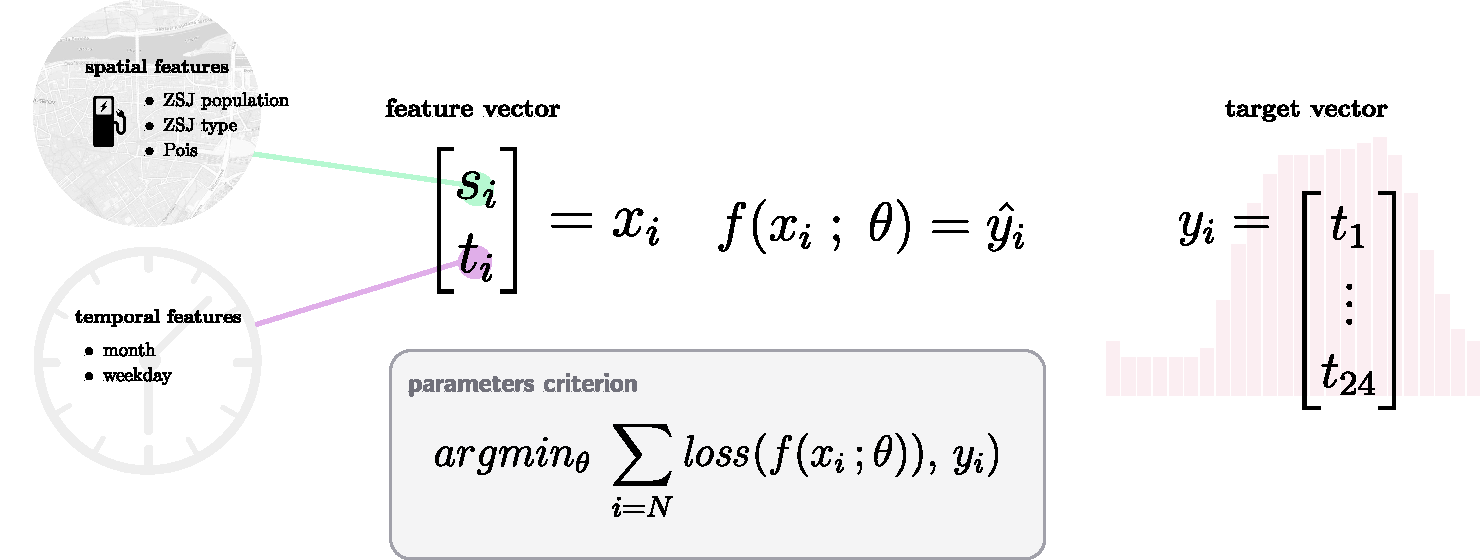
\includegraphics[width=1\textwidth]{diagram-detail}
    \caption[Problem modelling overview]{Problem approach overview}
\end{figure}

In this chapter, problem will be formulated together with model development and training. As a soluton to problem introduced in \ref{ch:intro}. That is, be able to predict potential demand for a new \acrfull{CP} placed anywhere in the city of Prague. As a solution a latent profile nerual network will be discussed which should be able to predict charging demand while also offer interpretability to its results.

\section{Problem statement}

\begin{marginfigure}
    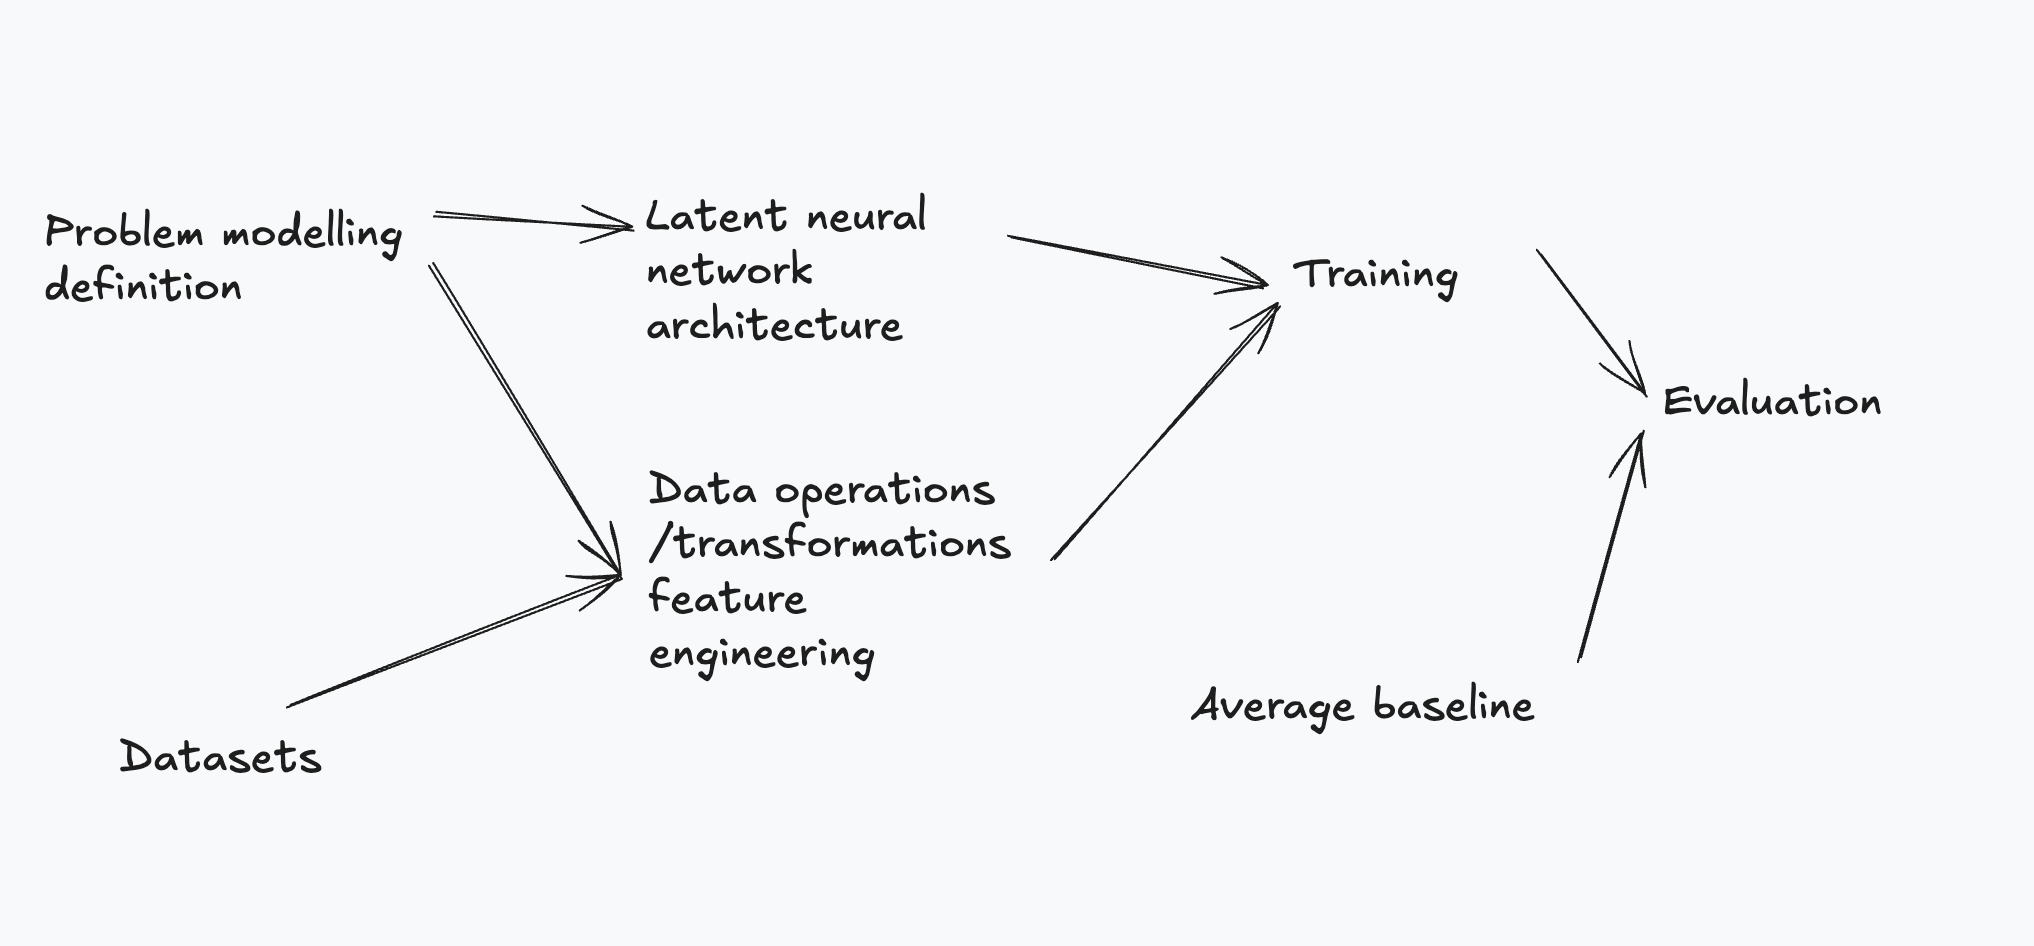
\includegraphics{diagram}
    \caption[Problem modelling overview]{Chapter content overview.}
\end{marginfigure}

Given existing charging sessions data and data landscape as described in \autoref{ch:data}. We are interested in predicting power demand for any new potential charger location in Prague as mentioned in \autoref{ch:problem}. Utilizing existing data.

\begin{itemize}
    \item define the data variables
    \item formulate the problem
    \item state possible solutions
    \item introduce latent profiles neural network model
    \item mention training procedure in all the detail, because everyone does this
    \item data normalization
    \item train test data split (based on location, to avoid double positions)
    \item loss function
    \item parameter tuning
\end{itemize}

\section{Architecture of the Latent Nerual Network}

\begin{figure}[hb]
    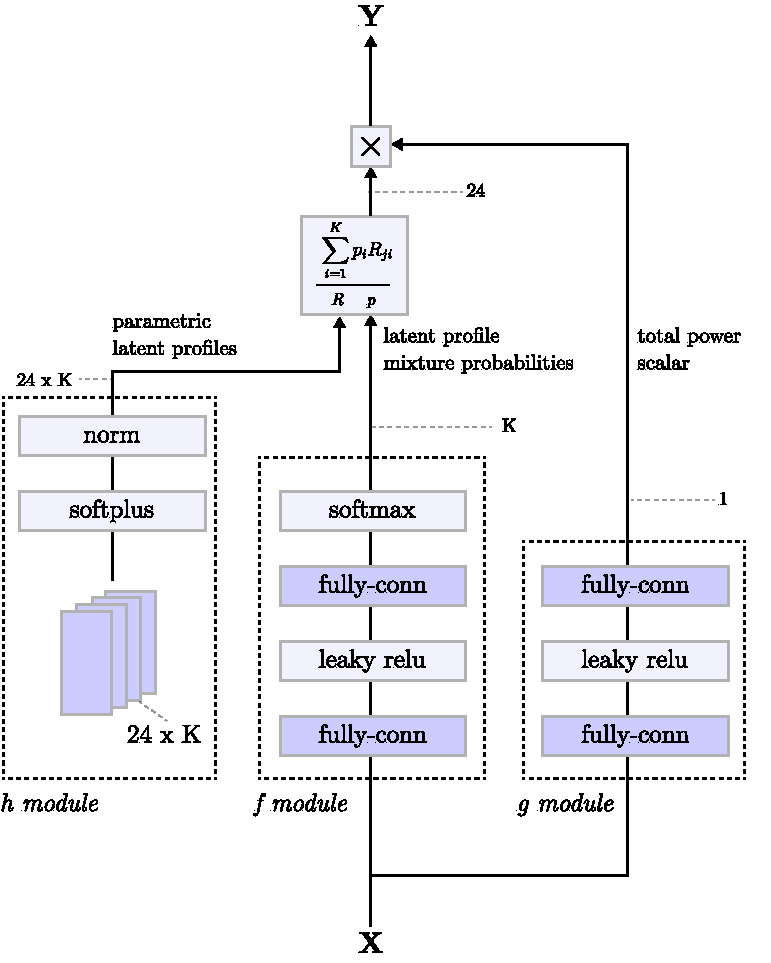
\includegraphics[width=0.7\textwidth]{nn-latent-architecture.pdf}
    \caption[Latent Neural Network Architecture]{Latent neural network architecture. Light blue rectangles denote NN layers without trainable parameters. While blue denotes layers with parameters learned by SGD. }
    \label{fig:nn-latent}
\end{figure}

\section{Input data transformation}

Standardization mainly.

\section{Training}


\section{Baseline}

To be able to tell if our results have some value.
Are we better than average ? Because noone has done it for prague and even our greenfield problem formulation.